\documentclass[a4paper,10pt]{article}
%\documentclass[a4paper,10pt]{scrartcl}

\usepackage[utf8]{inputenc}
% \usepackage{multicol}
\usepackage{fullpage}
% les figure imbriquées
\usepackage{epsfig}
\usepackage{subfigure}

\usepackage{graphicx}
\usepackage{amsmath}
\usepackage{amsthm}
\usepackage{amssymb}
\newtheorem{prop}{Propriété}
\newtheorem{algo}{Algorithme}
\newtheorem{defi}{Définition}

\title{Site Identification Decision Tree}
\date{}
\pdfinfo{%
  /Title    ()
  /Author   ()
  /Creator  ()
  /Producer ()
  /Subject  ()
  /Keywords ()
}

\begin{document}
\maketitle

% \section{Fonctionnement de l'algorithme}
\section{Description de l'algorithme}
On cherche à apprendre des sites provenant d'un graphe donné en entrée. Chaque site est indépendant.

\section{Découpe des sites}
Pour apprendre un graphe, on le découpe en sites de taille donnée (24 par défaut).
On effectue pour cela un parcours en largeur à partir de chaque noeud du graphe pour extraire un graphe partiel de type NGraph. Le type NGraph est constitué d'une matrice construite selon la numérotation obtenue avec le parcours en largeur, et d'une liste de symboles (pour chaque noeud).\\

L'exemple suivant est donné pour un parcours du graphe à partir du noeud~b. Lorsqu'il n'y a pas de fils (ou un seul), on place un 0 dans la matrice, sinon le numéro du noeud fils.

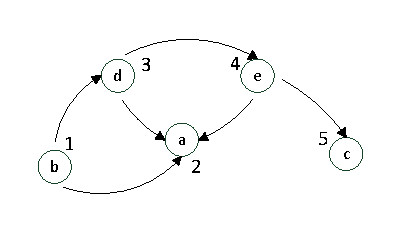
\includegraphics[width=0.60\textwidth]{src/img/graphesBFS5.pdf}
% &
$M_{i, j} = \begin{array}{r|cc}  & Fils 1 & Fils 2 \\
\hline
1 & 2 & 3\\
2 & 0 & 0\\
3 & 2 & 4\\ 
4 & 2 & 5\\ 
5 & 0 & 0\\ 
\end{array}$\\


% \begin{figure}[ht]
% \begin{center}
%   \subfigure[Graphe]{
% % \label{fig:CFGConstr}
% \epsfig{figure=images/graphesBFS5.pdf,height=5cm}}\quad
%   \subfigure[Matrice du NGraph]{
% % \label{fig:CFGNorm}
% $M_{i, j} = \begin{array}{r|cc}  & Fils 1 & Fils 2 \\
% \hline
% 1 & 2 & 3\\
% 2 & 0 & 0\\
% 3 & 2 & 4\\ 
% 4 & 2 & 5\\ 
% 5 & 0 & 0\\ 
% \end{array}$}
% \end{center}
% % \caption{Construction et normalisation du graphe de flot de contrôle}
% % \label{fig:CFGConstrNorm}
% \end{figure}

Une fois le site généré sous forme de NGraph, on va l'apprendre.

\section{Apprentissage d'un site}
\subsection{Construction de l'arbre de décision}
L'arbre de décision est constitué d'une racine qui est une noeud de décision (decisionNode) et de diverses informations sur les sites appris (valence, taille, ...).

\subsection{Noeud de décision et table de hashage}
Les noeuds de l'arbre de décision sont organisés en arbre depuis la racine, la décision du prochain noeud (fils) se fait sur la ligne de la matrice du site considéré comme suit (exemple avec le graphe précédent appris dans l'arbre).\\
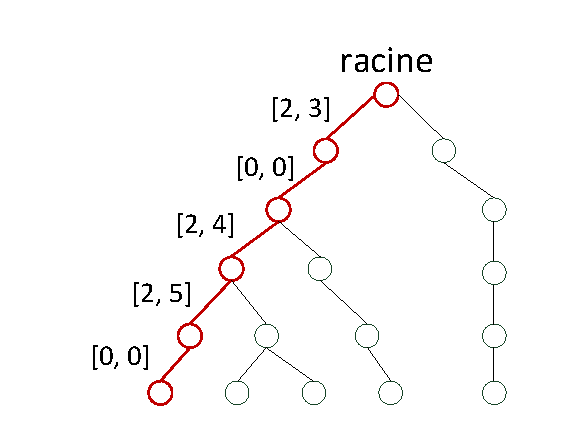
\includegraphics[width=0.6\textwidth]{src/img/arbredecision2.pdf}\\

Un noeud de décision est constitué d'une table de hashage pour la décision et d'un entier indiquant sa profondeur dans l'arbre.\\

Une table de hashage contient une liste d'éléments, chaque élément est constitué des valeurs déjà construites (par exemple 2 et 3 pour la première ligne), du noeud de décision vers lequel il pointe (fils), et du prochain élément (chaînage).\\

L'implémentation actuelle consiste à simplement avoir un élément dans la table de hashage et tous les élément chaînés. Il s'agit en fait d'une liste simple dans laquelle chercher les éléments déjà présents.

\subsection{Apprentissage}
Il suffit maintenant de placer le site dans l'arbre de décision. On le fait récusivement sur la ligne de la matrice du NGraph à apprendre en partant du noeud de décision racine en utilisant les hashtables.

\section{Détection}
Pour savoir si un site est déjà présent, on le transforme sous forme de NGraph, et on le cherche dans l'arbre en utilisant les hashtables.

\section{Usage}
Le programme prend en entrée des fichiers edge (.edg) fournis par sigtool.
\subsection{Comparer deux binaires}
\begin{verbatim}
./SIDT --learn openssl_byte.edg sality_layer1_v4.exe.edg
\end{verbatim}
Cette commande apprend openssl\_byte.edg et scanne sality\_layer1\_v4.exe.edg.

\subsection{Apprendre une liste de binaire, en scanner une autre}
Il suffit pour cela de construire un fichier avec les chemins des fichiers à apprendre (learn.lst) et un fichier avec ceux pour les fichiers à détecter (scan.lst), de la forme suivante :

% \begin{figure}
\begin{verbatim}
sality_layer1_v3.exe.edg
sality_layer3.exe.edg
sality_layer1_v4.exe.edg
\end{verbatim} 
% \end{figure}

Puis d'effectuer la commande suivante.
\begin{verbatim}
./SIDT --learn-list learn.lst scan.lst
\end{verbatim}

\section{TODO}
\begin{itemize}
 \item Sérialiser : permettre d'enregistrer la base dans un fichier, la charger
 \item Gestion de sites de différentes tailles (possible avec l'arbre de décision)
 \item Améliorer l'interface, les options
\end{itemize}



\end{document}
